%%%%%%%%%%%%%%%%%%%%%%%%%%%%%%%%%%%%%%%%%%%%%%%%%%%%%%%%%%%%%%%%%%%%%%%%%%%%%%%%
% Medium Length Graduate Curriculum Vitae
% LaTeX Template
% Version 1.2 (3/28/15)
%
% This template has been downloaded from:
% http://www.LaTeXTemplates.com
%
% Original author:
% Rensselaer Polytechnic Institute 
% (http://www.rpi.edu/dept/arc/training/latex/resumes/)
%
% Modified by:
% Daniel L Marks <xleafr@gmail.com> 3/28/2015
% 
% Further modified by:
% Rohan Bavishi <rohan.bavishi95@gmail.com> 9/20/2016
%
% Further modified by:
% Nicolas Badoux <n.badoux@hotmail.com> 11/3/2018
%
% Important note:
% This template requires the simple_style.cls file to be in the same directory 
% as the .tex file. The res.cls file provides the resume style used for 
% structuring the document.
%
%%%%%%%%%%%%%%%%%%%%%%%%%%%%%%%%%%%%%%%%%%%%%%%%%%%%%%%%%%%%%%%%%%%%%%%%%%%%%%%%

%-------------------------------------------------------------------------------
%	PACKAGES AND OTHER DOCUMENT CONFIGURATIONS
%-------------------------------------------------------------------------------

%%%%%%%%%%%%%%%%%%%%%%%%%%%%%%%%%%%%%%%%%%%%%%%%%%%%%%%%%%%%%%%%%%%%%%%%%%%%%%%%
% You can have multiple style options the legal options ones are:
%
%   centered:	the name and address are centered at the top of the page 
%				(default)
%
%   line:		the name is the left with a horizontal line then the address to
%				the right
%
%   overlapped:	the section titles overlap the body text (default)
%
%   margin:		the section titles are to the left of the body text
%		
%   11pt:		use 11 point fonts instead of 10 point fonts
%
%   12pt:		use 12 point fonts instead of 10 point fonts
%
%%%%%%%%%%%%%%%%%%%%%%%%%%%%%%%%%%%%%%%%%%%%%%%%%%%%%%%%%%%%%%%%%%%%%%%%%%%%%%%%

\documentclass[mm, 11pt]{simple_style}  

% Default font is the helvetica postscript font
\usepackage{helvet}
\usepackage[hidelinks]{hyperref}
\usepackage{url}
\usepackage[utf8]{inputenc}
\usepackage[T1]{fontenc}
\usepackage[a4paper, left=12mm, right=45mm, top=15mm, bottom=15mm]{geometry}
\usepackage[fristpage=true, color=black, opacity=0.5, angle=90]{background}

\begin{document}

\newsectionwidth{26mm}
%-------------------------------------------------------------------------------
%	NAME AND ADDRESS SECTION
%-------------------------------------------------------------------------------
\name{Nicolas Badoux}
%\qualification{Senior undergraduate ETHZ student}
\emailone{n.badoux@hotmail.com}
\emailtwo{nicolas.badoux@epfl.ch}
%\website{https://nicolasbadoux.com}{\url{nicolasbadoux.com}}
%\github{https://github.com/vwvw}{\url{github.com/vwvw}}
\phone{+41 79 914 00 47}
\linkedin{nbadoux}
\citizenship{Swiss citizen---married}
\birthdate{Born in 1994}
\address{\href{https://maps.app.goo.gl/kmh2wtaNsmxrcqGc8}{Rue de la Gare 21}
&\multirow{3}{*}{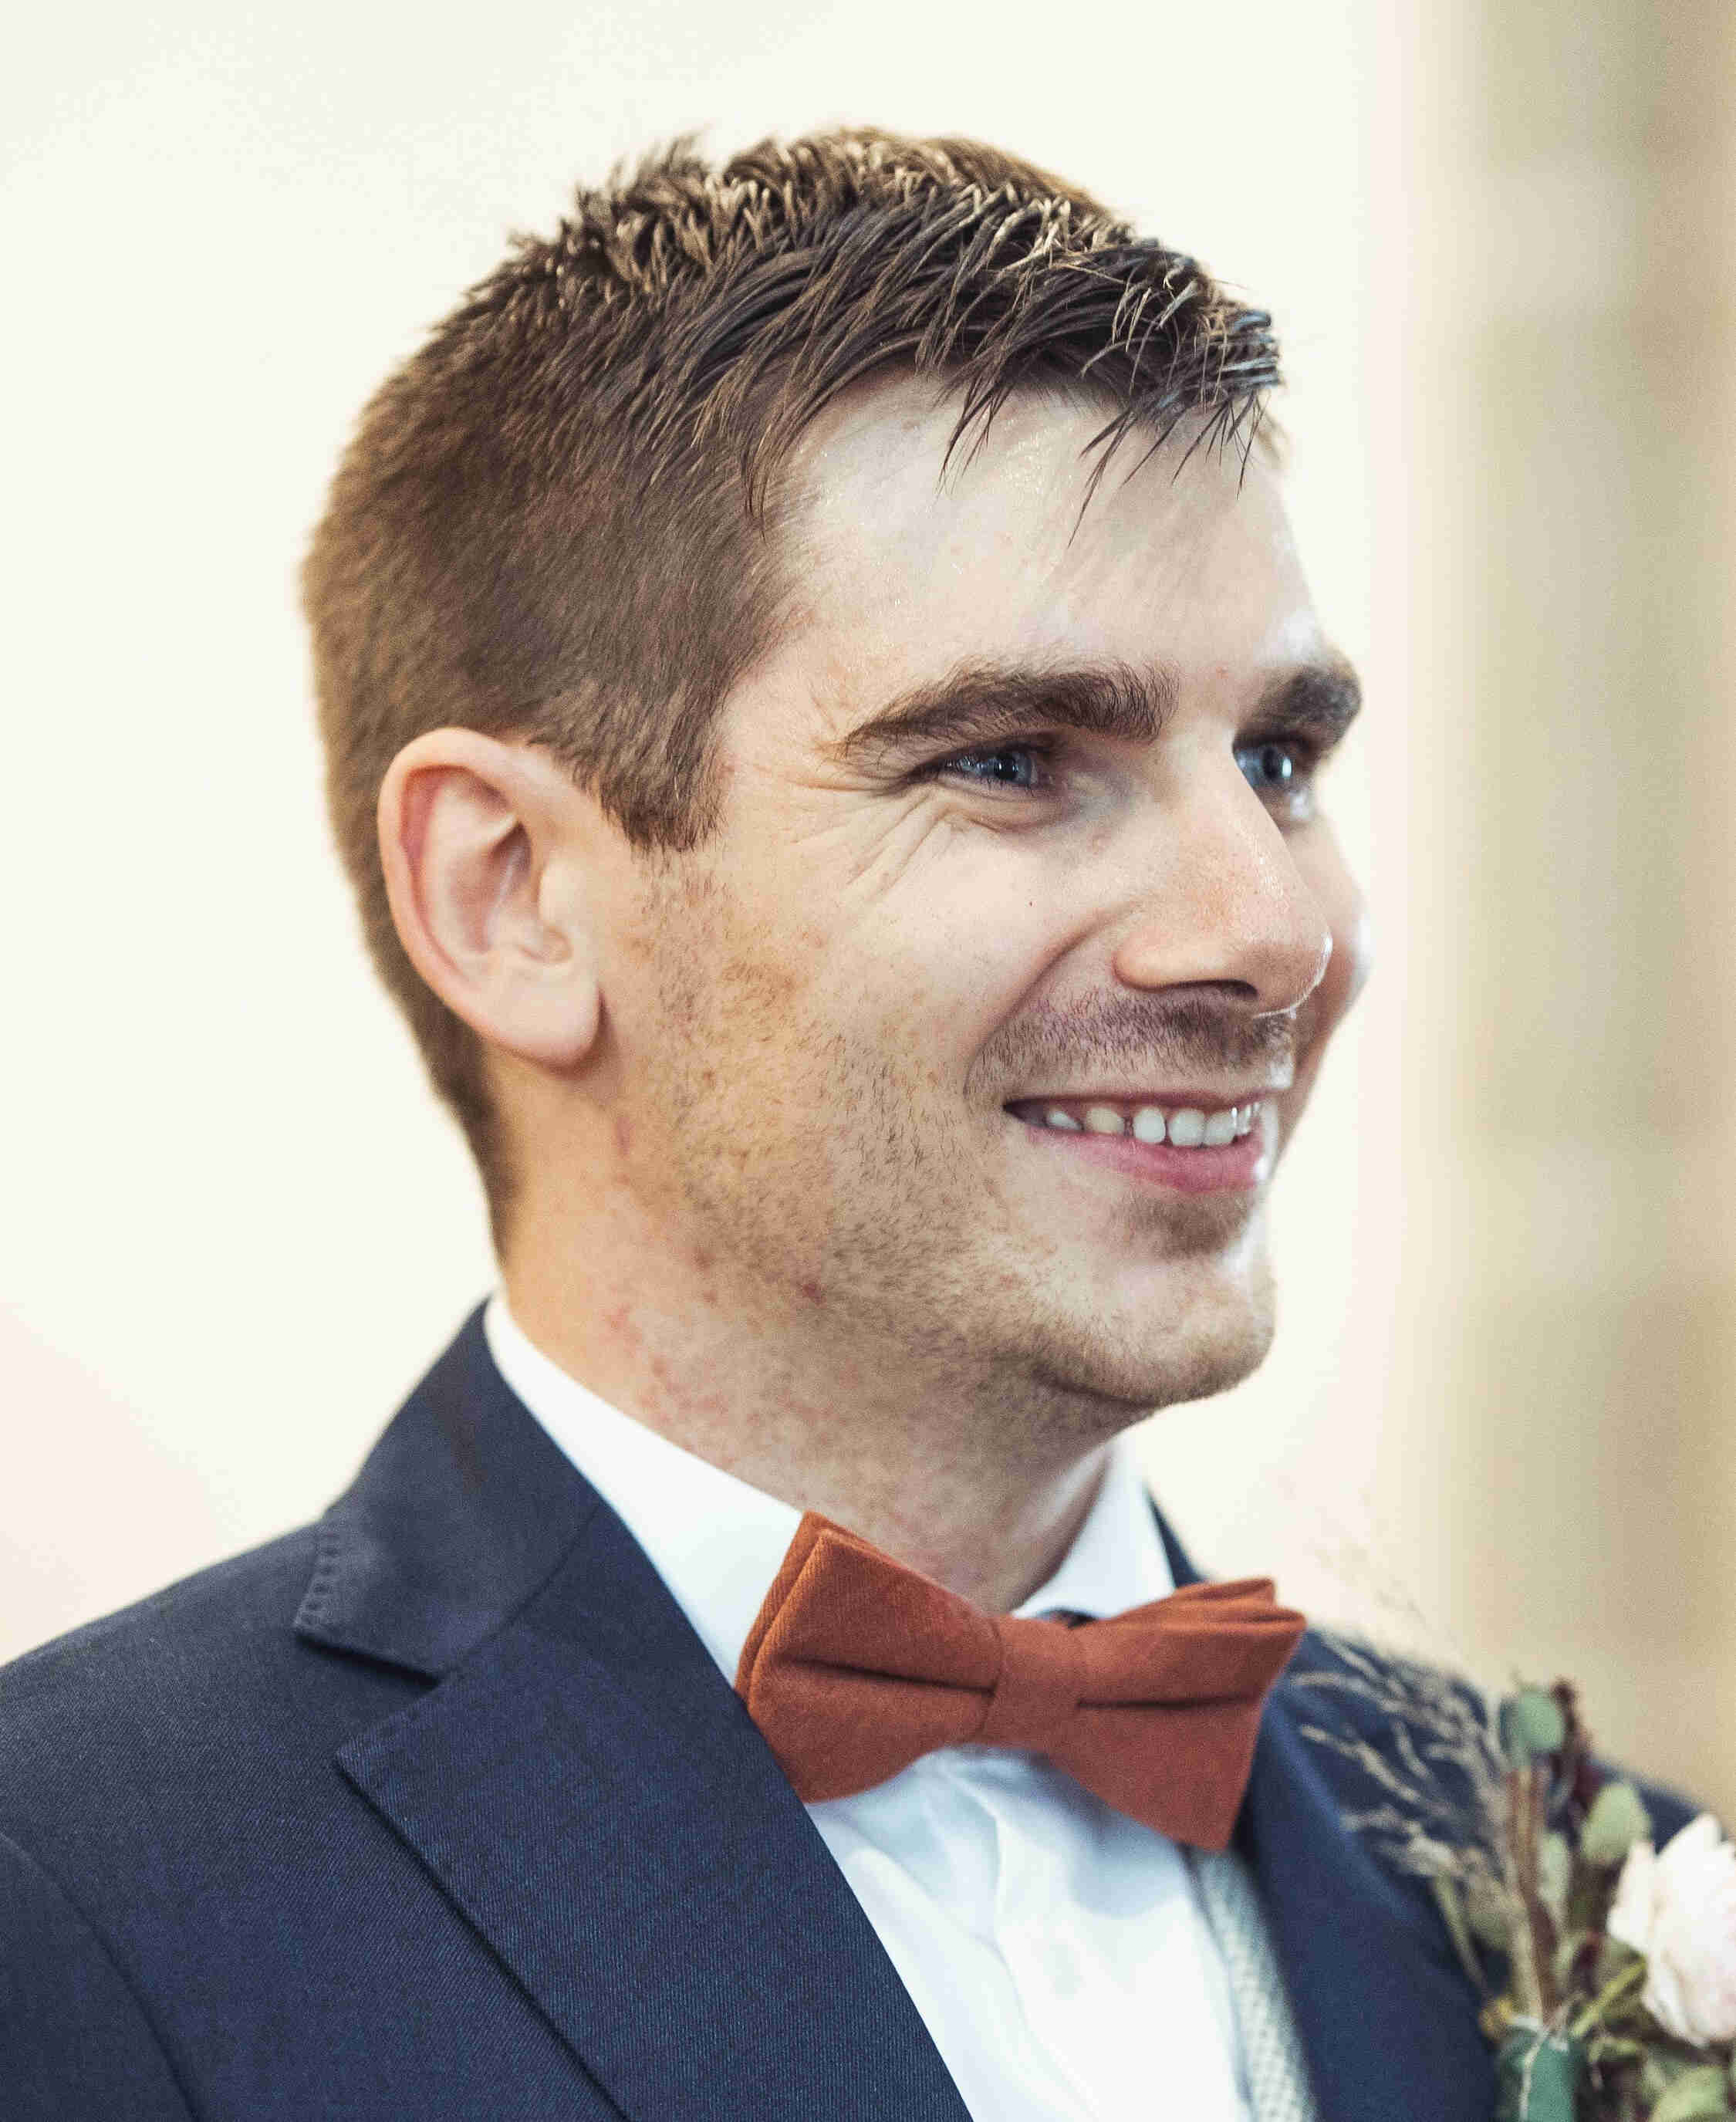
\includegraphics[height=2.1cm]{photo.jpg}}\\
         \href{https://maps.app.goo.gl/kmh2wtaNsmxrcqGc8}{1030} 
         \href{https://maps.app.goo.gl/kmh2wtaNsmxrcqGc8}{Bussigny}\\
         \href{https://maps.app.goo.gl/kmh2wtaNsmxrcqGc8}{CH---Switzerland}
}

\begin{resume}
%-------------------------------------------------------------------------------
%-------------------------------------------------------------------------------
%	WORK SECTION
%-------------------------------------------------------------------------------
\section{Statement of Purpose}

Passionate about cybersecurity, its ever evolving nature, and the adaptations it requires.\\
%Constant curiosity for complex systems to understand their weak points. 
%My natural curiosity drives me to spot and try to understand odd patterns in software.\\
Pushing for a shift of security left in the SDLC through threat modelling and secure DevOps.\\
With automated defenses and monitoring, I hope to reduce the repercussion of cyber incidents.\\
%I believe that security of complex systems can be improved.
% highlight how I want to push each collaborator to their full potential and that it's how I think a team is most effective.
Can-do attitude, committed, and strong ability to adapt to changing requirements.\\
%looking for a collaborative environment where I can continue learning.
%Striving to devise fixes and defenses against bugs through automation and secure foundations.
%
\sectionline

\section{Experience}
\begin{position}
    \employer{\href{https://hexhive.ch}{EPFL}}
    \title{Doctorate of Sciences (PhD)}
    \location{Lausanne, CH}
    \duration{Mar' 2020--May 2025}
    \description{
      \item Lead the development and evaluation of different security-themed
      projects reducing the attack surface of low-level code (C/C++). With novel
      secure dialects, compiler passes (SAST) and automated testing (DAST), we
      ease secure development across large code bases.
      \item As part of our research, we extensively tested low/level APIs and
      dutifully followed the vulnerability lifecycle, from responsible
      disclosure to contribution of fixes.
      %
      \item Facing continuously evolving requirements, I strategically scoped our
      projects and effectively communicated their outcomes to a global audience.
      %
      \item In a diverse team, I collaborated with senior professors and designed and mentored
      research projects for junior students. We contributed to open source projects and reported CVEs.
    }
\end{position}
\begin{position}
    \employer{\href{https://digger.ch}{Fondation Digger}\normalfont{, NGO}}
    \title{Software Engineer}
    \location{Tavannes, CH}
    \duration{Aug' 2019--Mar' 2020}
    \description{
      \item Quantified the feasibility of low-latency VR in C++ for an 
      \href{https://digger-dtr.com/en/products/digger-scraper/}{industrial demining machinery}.
    }
\end{position}
\begin{position}
    \employer{\href{https://compassion.ch}{Compassion Suisse}\normalfont{, NGO}}
    \title{Software Engineer}
    \location{Yverdon, CH}
    \duration{Mar'--May 2018}
    \description{
        \item Contributed in an Agile environment to
        \href{https://github.com/CompassionCH/compassion-switzerland}{open source}
        modules for the Python \href{https://www.odoo.com/}{Odoo ERP}.
    }
\end{position}
\begin{position}
    \employer{\href{https://ergon.ch/en}{Ergon Informatik}}
    \title{Security Engineer Intern}
    \location{Z\"urich, CH}
    \duration{60\%---Sept' 2017--Mar' 2018}
    \description{
        \item Designed and developped a blackbox fuzzer for testing a
        \href{https://www.airlock.com/en/products/airlock-waf/}{Web Application
        Firewall (WAF)}.
    }
\end{position}
\begin{position}
    \employer{\href{https://www.morganstanley.com/}{Morgan Stanley}}
    \title{Technology Summer Analyst}
    \location{London, UK}
    \duration{Jun'--Aug' 2016}
    \description{
        \item Developed a webview for metrics tracked by the Architecture Security team of the bank.
    }
\end{position}
\vspace{-\parskip}
\sectionline
%-------------------------------------------------------------------------------
\section{Education}

\cusemph{Doctor of Sciences (PhD)}
\timeline{2020--\textit{2025}}\\
\textsl{\href{https://ic.epfl.ch/en}{\'Ecole Polytechnique F\'ed\'erale de Lausanne (EPFL)}} - Switzerland
\begin{itemize}
  \item Advisor: \href{https://nebelwelt.net/}{Prof. Mathias Payer} in the \href{https://hexhive.epfl.ch}{HexHive} laboratory.
  \item \href{https://infoscience.epfl.ch/entities/publication/5c91711a-5bf2-4fe0-b04e-830ac3a13bfb}{Thesis: Securing low-level code with minimal developer efforts.}
  \item Keywords: System security, software testing, compiler-based defenses, fuzzing. 
\end{itemize}


%-------------------------------------------------------------------------------
\cusemph{Master of Science ETH in Computer Science}
\timeline{2016--2019}\\
\textsl{\href{https://www.inf.ethz.ch/}{Eidgen\"ossische Technische Hochschule Z\"urich (ETHZ)}} - Switzerland

\begin{itemize}
  \item  Specialization in Information Security, GPA: 5.39/6.
\end{itemize}
%-------------------------------------------------------------------------------
\cusemph{Bachelor in Communication Sciences}
\timeline{2013--2016}\\
\textsl{\href{https://ic.epfl.ch/en}{\'Ecole Polytechnique F\'ed\'erale de Lausanne (EPFL)}} - Switzerland

\begin{itemize}
  \item \textbf{Exchange program} @
\textit{\href{https://www.ece.cmu.edu/}{Carnegie Mellon University}} - USA, GPA: 5.26/6.
\timeline{2015--2016\hspace{-1em}}
\end{itemize}
%-------------------------------------------------------------------------------
\cusemph{Billingual Matura (German/French)}
\timeline{2010--2013}\\
\textsl{\href{https://www.kanti-frauenfeld.ch/}{Kantonschule Frauenfeld} \& Gymnase d'Yverdon} - Switzerland

\begin{itemize}
  \item Specialization in Mathematics and Physics, GPA: 5.19/6, Best 3\%.
\end{itemize}

\sectionline
%-------------------------------------------------------------------------------
%  SKILLS SECTION
%-------------------------------------------------------------------------------
\section{Skills}
\cusemph{Programming Languages}: Python, C++, \LaTeX, Bash.

\cusemph{Software}: LLVM, Docker, GDB, Linux, Make, afl++, libfuzzer.

\cusemph{Spoken Languages}: French (native), English (C2), Swiss-German (C2), German (C1).

\pagebreak
\sectionline
%-------------------------------------------------------------------------------
%-------------------------------------------------------------------------------
%	RESEARCH SECTION
%-------------------------------------------------------------------------------
\section{Research Projects}
\begin{research}
    \title{\href{https://hexhive.epfl.ch/publications/files/25NDSS.pdf}{\texttt{type++}:
    prohibiting type confusion with inline type information}}
    \location{\href{https://www.ndss-symposium.org/ndss2025/}{NDSS'25}}
    \authors{\textbf{Nicolas Badoux}, Flavio Toffalini, Yuseok Jeon, \& Mathias Payer.}
    \description{%
      \item \textit{Distinguished Paper Award} (top 1\% of submissions).
      %
      \item In
      C++, incorrect downcasts are a severe vulnerability often exploited in the
      wild.
      %
      \item By inlining the type in each C++ object, we create a compiler-based
      mitigation against type confusion attacks allowing downcast to be checked
      at runtime while requiring minimal code adaptations. We evaluate our
      prototype against the state-of-the-art and achieve less than 1\% runtime
      overhead while protecting 90B casts. We deploy our prototype on Chromium.
      %
      \item Built on top of LLVM, \texttt{type++} is available on \href{https://github.com/HexHive/typepp}{\underline{GitHub}} and its artifact evaluated.%
      %
      \item During this multi-year project, I learned some intricacies of
      compilers, developed my writing skills, and  strategic planning to face a
      constantly evolving project. 
      %
    }
\end{research}
\begin{research}
    \title{\href{https://nebelwelt.net/files/25FSE2.pdf}{\textsc{libErator}: Balancing library fuzzing without consumer code}}
    \location{\href{https://conf.researchr.org/home/fse-2025}{FSE'25}}
    \authors{Flavio Toffalini, \textbf{Nicolas Badoux}, Zurab Tsinadze, \& Mathias Payer.}
    \description{%
      \item Drivers, a sequence of API calls building state, allows for dynamic
      testing like fuzzing, to execute a library's code. Manually written
      drivers are rare and exhaustively tested.
      % 
      \item \textsc{libErator} automates the generation of fuzzing drivers
      without consumer code and allows for balancing resources between driver
      generation and fuzzing.
      %
      \item From insights gathered through LLVM passes, we build valid C drivers
      calling the API.
      %
      \item We report and fix 24 bugs, including
      \href{https://nvd.nist.gov/vuln/detail/cve-2024-8006}{CVE-2024-8006}. We release our prototype on \underline{\href{https://github.com/HexHive/liberator}{Github}}.
      %
      \item Through the design and multifaceted evaluation of \textsc{libErator}, I improved my cross-cutting understanding of complex systems.  
      %
    }
\end{research}
\begin{research}
    \title{\href{https://nebelwelt.net/files/25DIMVA.pdf}{Sourcerer: channeling the void}}
    \authors{\textbf{Nicolas Badoux}, Flavio Toffalini, \& Mathias Payer.}
    \location{\href{https://www.dimva.org/dimva2025/}{DIMVA'25}}
    \description{%
      \item In C++, conversions from \texttt{void*} to typed pointers are ubiquitous but,
      if the type is not the original one, leads to type confusions and possibly
      further memory corruption.
      %
      \item By extending the protection of type++ to all the types used in
      casts, we design Sourcerer, a complete type confusions sanitizer. With a
      low-overhead of 5\% on average, we conduct the first fuzzing
      campaign targeting specifically type confusions. 
      %
      \item We find type confusions in Blender and OpenCV and release our prototype on \href{https://github.com/HexHive/Sourcerer}{\underline{GitHub}}. 
      %
      \item As the main author, I designed and evaluated our system as well as wrote the paper.
      %
      }
\end{research}
\vspace{-\parskip}
\sectionline

%-------------------------------------------------------------------------------
%  TEACHING SECTION
%-------------------------------------------------------------------------------
\section{Teaching Assistant}
%


\cusemph{Operating System} \textit{(2021)}
\cusemph{Software Security} \textit{(2021 \& 2023)}
\cusemph{Information, Calcul \& Communication} \textit{(2022 \& 2024)}
\cusemph{Information Security \& Privacy} \textit{(2023)}

\sectionline
%\section{Talks}
%
%\cusemph{NDSS'25} - \texttt{type++}: prohibiting type confusion with inline type information \timeline{2025}
%
%\sectionline
%-------------------------------------------------------------------------------

%-------------------------------------------------------------------------------
%	Interests
%-------------------------------------------------------------------------------
\section{Activities}
\begin{extra}
  \title{Board Member, Treasurer \textnormal{-
  \href{https://www.gbeu.ch}{Groupes Bibliques des Écoles et Universités}}}
  \location{2023--ongoing}
  \description{%
    \item Define the vision, hiring, and budget planning ($\simeq$ 500kCHF).
  }
\end{extra}
\begin{extra}
  \title{Camp Leader \textnormal{-
  \href{https://www.interjeunes.net/explosion-camp}{Interjeunes} \&
  \href{https://ligue.ch}{Ligue pour la Lecture de la Bible}}}
  \location{2014, 2017, 2021, 2022}
  \description{
    \item Lead week-long camps with up to 110 kids/young adults. Built a team,
    prepared the event, managed the team and had final authority.
  }
\end{extra}

\sectionline
\section{References}
\begin{extra}
  \title{\href{https://nebelwelt.net/}{Prof. Dr. Mathias Payer}}
  \location{\href{mailto:mathias.payer@nebelwelt.net}{mathias.payer@nebelwelt.net}}
  \description{%
    \item \href{https://nebelwelt.net/}{Associate Professor at EPFL in Lausanne
    (CH)} and head of \href{https://www.hexhive.epfl.ch}{HexHive}.
    %
    \item Advised me during my PhD between 2020 and 2025. 
  }
\end{extra}
\begin{extra}
  \title{\href{https://flaviotoffalini.info/}{Prof. Dr. Flavio Toffalini}}
  \location{\href{mailto:flavio.toffalini@rub.de}{flavio.toffalini@rub.de}}
  \description{
    \item \href{https://flaviotoffalini.info/}{Assistant Professor at Ruhr-Universität} in Bochum (DE).
    \item Close collaborator and advising post-doc during my PhD (2021--2025). 
  }
\end{extra}
\begin{extra}
  \title{Benoît Pfister}
  \location{\href{mailto:benoit.pfister@gbeu.ch}{benoit.pfister@gbeu.ch}}
  \description{
    \item Chairman of the Board at Groupes Bibliques des Écoles et Universités. 
    \item We worked together for hiring committees, budgeting, and general strategy.
  }
\end{extra}

\end{resume}
\end{document}
